% Load preamble
\documentclass[../main.tex]{subfiles}

\begin{document}

\subsection{Stavový opis}

Stavový opis je jedna z foriem opisu dynamického lineárneho systému. Základom je definovanie vnútorných stavov systému, ako sa tieto stavy menia v čase a ako vyzerá výstup zo systému.
	
\begin{equation}
	\begin{split}
		\dot{x} = Ax + Bu \\
		y = Cx + Du
	\end{split}
	\label{eqn:matz_stavovaRovnica}
\end{equation}

Pre SISO systémy je C vektor (riadkový) a D skalár. Pre MIMO systémy je C matica a D je vektor (stĺpcový). Majme systém opísaný rovnicami \ref{eqn:matz_system}.

\begin{equation}
	\begin{split}
		\dot{x_1} =& x_2 \\
		\dot{x_2} =& x_3 \\
		\dot{x_3} =& -x_1 + 8x_2 + 3x_3 - 6u \\
		y =& x_1
	\end{split}
	\label{eqn:matz_system}
\end{equation}

Tento systém môžeme napísať aj v maticovom tvare:

        \begin{center}
		$\begin{bmatrix} 
			\dot{x_1} \\ 
			\dot{x_2} \\ 
			\dot{x_3} \\ 
		\end{bmatrix}  = 
		\begin{bmatrix} 
			0 & 1 & 0 \\ 
			0 & 0 & 1 \\ 
			-1 & 8 & 3 \\ 
		\end{bmatrix} 
		\begin{bmatrix} 
			x_1 \\ 
			x_2 \\ 
			x_3 \\ 
		\end{bmatrix} +
		\begin{bmatrix} 
			0 \\ 
			0 \\ 
			-6 \\ 
		\end{bmatrix}
		u $
	\label{eqn:matz_system2}
        \end{center}

        \begin{center}
		$y  = 
		\begin{bmatrix} 
			1 & 0 & 0 \\ 
		\end{bmatrix} 
		\begin{bmatrix} 
			x_1 \\ 
			x_2 \\ 
			x_3 \\ 
		\end{bmatrix} +
		0u $
	\label{eqn:matz_system2}
        \end{center}

Laplaceovu transformáciu získame rovnice \ref{eqn:matz_systemLap}. 

\begin{equation}
	\begin{split}
		Ys^3 = -Y + 8 Ys + 3Ys^2 - 6U
	\end{split}
	\label{eqn:matz_systemLap}
\end{equation}

\begin{equation}
	\begin{split}
		Y(s^3 -3s^2 -8s + 1) = - 6U
	\end{split}
\end{equation}

\begin{equation}
	\begin{split}
		\frac{Y}{U} = \frac{-6}{s^3 -3s^2 -8s + 1} = G(s)
	\end{split}
	\label{eqn:matz_systemPrenos}
\end{equation}

Rovnica  \ref{eqn:matz_systemPrenos} predstavuje prenosovú funkciu nášho systému.

Simulačná schéma je na obr. \ref{fig:matz_systemStavovyOpisSimulink}. V bloku integrátor je možné nastaviť počiatočne hodnoty stavov (počiatočné podmienky). Pri tejto schéme je dôležité uvedomiť si dimenzie jednotlivých signálov.

\begin{figure}[h!]
	\centering
	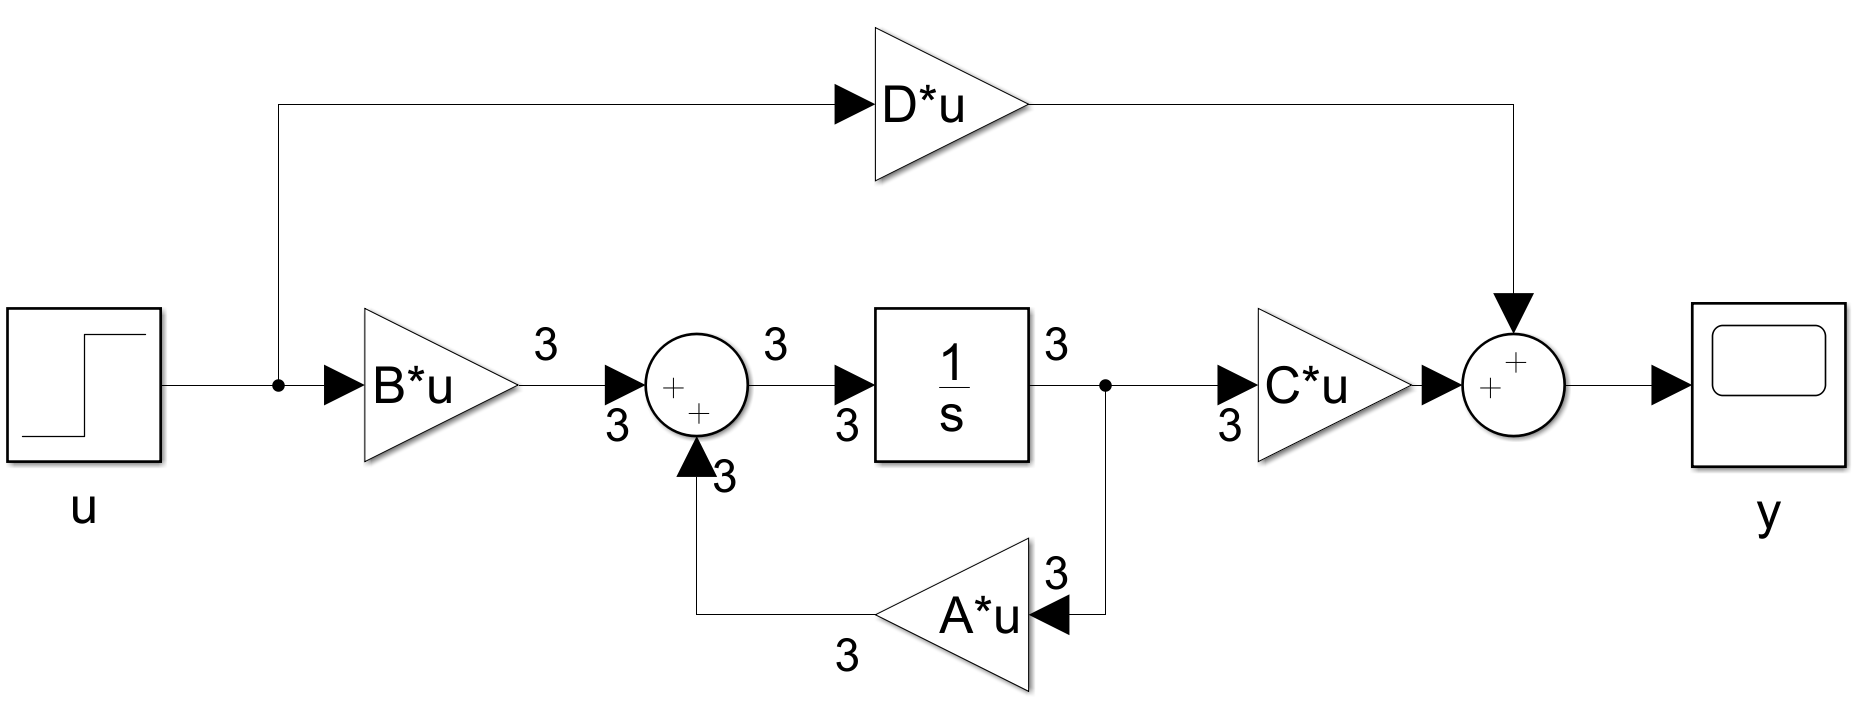
\includegraphics[width=0.8\linewidth]{matzaklady/SchemaStavovyOpis}
	\caption{Simulačná schéma systému definovaná pomocou stavového opisu}
	\label{fig:matz_systemStavovyOpisSimulink}
\end{figure}

\subsection{Rovnvoažné stavy}
	
\subsection{Linearizácia}

Linearizácia je proces, pri ktorom z nelineárneho systému spravíme lineárny. Tento lineárny systém opisuje pôvodný systém "presne" len v okolí pracovného bodu. Veľkosť tohto okolia záleží od priebehu funkcií. Používa sa pri tom rozvoj do Taylorovho radu (rovnica \ref{fig:matz_systemStavovyOpisSimulink}), kedy použijeme len prvý člen.

\begin{equation}
	\begin{split}
		f(x) \approx \sum^{inf}_{n=0}{\frac{f^{(n)}(a)}{n!}(x-a)^n}
	\end{split}
	\label{eqn:matz_taylorovRad}
\end{equation}

Kde $f^{(n)}$ je $n$-tá derivácia funkcie $f$ v bode $a$, v prípade funkcie viacerých premenných je to gradient. Funkcia $f$ musí byť diferencovatelná.

\begin{equation}
	\begin{split}
		f(x) \approx \frac{f^{(1)}(x)}{1!}(x-x_0)^1 = \frac{\partial{f}}{\partial{x}}|_{a}(x-x_0) = \nabla{f}|_{a}\Delta{x}
	\end{split}
	\label{eqn:matz_prvyClenTaylorovhoRadu}
\end{equation}

Majme systém opísaný rovnicami \ref{eqn:matz_rovniceSystemu}. Keďže sa tam vyskytujú aj nelineárne členy (sínus, kosínus a ich súčin), tento systém je nelineárny. Pri linearizácií tohto systému musíme počítať gradient každej rovnice podľa stavového vektora a vstupov, ďalej len vektora parametrov funkcií $x$. Nech bod P [0 0 0 0] je pracovným bodom, v ktorom budeme systém linearizovať.
\begin{center}
$x = \begin{bmatrix}
\Delta{x_1} \\
\Delta{x_2} \\
\Delta{x_3} \\
\Delta{u}
\end{bmatrix}$
\end{center}

\begin{equation}
		\begin{aligned}
		\dot{x_1} &= x_1 + x_2 - x_3 + sin(x_2) 			\\
		\dot{x_2} &= - x_1 - x_2 						\\
		\dot{x_3} &= cos(x_2) (sin(x_2) - x_3) - u 	\\
		y &= x_1
		\end{aligned}
		\label{eqn:matz_rovniceSystemu}
\end{equation}

\begin{equation}
		\begin{aligned}
		\nabla{\dot{x_1}} &= [\frac{\partial{\dot{x_1}}}{\partial{x_1}},\frac{\partial{\dot{x_1}}}{\partial{x_2}},\frac{\partial{\dot{x_1}}}{\partial{x_3}},\frac{\partial{\dot{x_1}}}{\partial{u}}] = [1, 1 + cos(x_2), -1, 0]			\\
		\nabla{\dot{x_2}} &= [\frac{\partial{\dot{x_2}}}{\partial{x_1}},\frac{\partial{\dot{x_2}}}{\partial{x_2}},\frac{\partial{\dot{x_2}}}{\partial{x_3}},\frac{\partial{\dot{x_2}}}{\partial{u}}] = [-1, -1, 0, 0]			\\
		\nabla{\dot{x_3}} &= [\frac{\partial{\dot{x_3}}}{\partial{x_1}},\frac{\partial{\dot{x_3}}}{\partial{x_2}},\frac{\partial{\dot{x_3}}}{\partial{x_3}},\frac{\partial{\dot{x_3}}}{\partial{u}}] = [0, -sin^2(x_2)+cos^2(x_2), -cos(x_2), -1]			\\
		y &= [\frac{\partial{y}}{\partial{x_1}},\frac{\partial{y}}{\partial{x_2}},\frac{\partial{y}}{\partial{x_3}},\frac{\partial{y}}{\partial{u}}] = [1, 0, 0, 0]			\\
		\end{aligned}
		\label{eqn:matz_rovniceSystemuGradient}
\end{equation}

Gradient v pracovnom bode dostaneme dosadením hodnôt pracovného bodu.

\begin{equation}
		\begin{aligned}
		\nabla{\dot{x_1}}|_{P} &= [1, 1 + cos(0), -1, 0] = [1, 2, -1, 0]			\\
		\nabla{\dot{x_2}}|_{P} &= [-1, -1, 0, 0] \\
		\nabla{\dot{x_3}}|_{P} &= [0, -sin^2(0)+cos^2(0), -cos(0), -1] = [0,1, -1, -1]			\\
		\nabla{y}|_{P} &= [1, 0, 0, 0]			\\
		\end{aligned}
		\label{eqn:matz_rovniceSystemuGradient}
\end{equation}

Ak vynásobíme gradienty v pracovnom bode vektorom $x$, dostaneme linearizovanú sústavu diferenciálnych rovníc, ktoré opisujú správanie sa systému v okolí pracovného bodu $P$, rovnice \ref{eqn:matz_rovniceLinearnySystem}.

\begin{equation}
		\begin{aligned}
		\Delta{\dot{x_1}} &= \Delta{x_1} + 2\Delta{x_2} - \Delta{x_3}			\\
		\Delta{\dot{x_2}} &= -\Delta{x_1} - \Delta{x_2} \\
		\Delta{\dot{x_3}} &= \Delta{x_2} - \Delta{x_3} - \Delta{u}		\\
		\Delta{y} &= \Delta{x_1}			\\
		\end{aligned}
		\label{eqn:matz_rovniceLinearnySystem}
\end{equation}



	
\subsection{Riešenie preurčenej sústavy rovníc}

Preurčená sústava rovníc, obsahuje viac rovníc ako neznámych premenných. Pri riešení preurčene sústavy rovníc použijeme metódu najmenších štvorcov. Pomocou metódy najmenších štvorcov sa budeme snažiť aproximovať riešenie $x$ preurčenej sústavy rovníc \ref{eqn:MaticovyZapisPSR}.

\begin{equation}
	Ax \approx b
	\label{eqn:MaticovyZapisPSR}
\end{equation}

Uvažujeme nasledovnú preurčenú sústavu rovníc:

\begin{equation}
	\begin{split}
	 x+y  & = 5 \\
	 2x+4y+10 & = 8 \\
	 x+5y & = 15 \\
	 -2x+4y+10 & = 8 \\
	\end{split}
	\label{eqn:PreurcenySystem}
\end{equation}

Preurčenú sústavu rovníc \ref{eqn:PreurcenySystem} môžeme maticovo zapísať v tvare:
\begin{equation}
\begin{bmatrix} 1 & 1\\ 2 & 4 \\1 &5 \\-2& 4\end{bmatrix}\begin{bmatrix}x \\y \end{bmatrix} = \begin{bmatrix} 5 \\-2\\15\\-2 \end{bmatrix}
 \label{eqn:MaticovyZapisPiklad}
\end{equation}

Na výpočet neznámych premenných x,y použijeme metódu najmenších štvorcov :
\begin{equation}
	\begin{split}
	\begin{bmatrix}x \\y \end{bmatrix} &=  (A^TA)^{-1}A^Tb\\
	\begin{bmatrix}x \\y \end{bmatrix} &=  \begin{bmatrix} 1.4265 \\0.9559\end{bmatrix}
	\end{split}
	\label{eqn:MNS}
\end{equation}

		
\end{document}
